\documentclass[a4paper,12pt]{article}

\usepackage[T2A]{fontenc}			
\usepackage[utf8]{inputenc}			
\usepackage[english,russian]{babel}	

\usepackage[
bookmarks=true, colorlinks=true, unicode=true,
urlcolor=black,linkcolor=black, anchorcolor=black,
citecolor=black, menucolor=black, filecolor=black,
]{hyperref}

\usepackage{color}
\usepackage{caption}
\DeclareCaptionFont{white}{\color{black}}
\DeclareCaptionFormat{listing}{\colorbox{white}{\parbox{\textwidth}{#1#2#3}}}
\captionsetup[lstlisting]{format=listing,labelfont=white,textfont=white}

\usepackage{amsmath,amsfonts,amssymb,amsthm,mathtools} 
\usepackage{wasysym}

\usepackage[cache=false]{minted}

\usepackage{graphicx}
%\usepackage[cache=false]{minted}
\usepackage{cmap}
\usepackage{indentfirst}

\usepackage{listings} 
\usepackage{fancyvrb}

\usepackage{geometry}
\geometry{left=2cm}
\geometry{right=1.5cm}
\geometry{top=1cm}
\geometry{bottom=2cm}

\setlength{\parindent}{5ex}
\setlength{\parskip}{0.5em}

\usepackage{pgfplots}

\usepackage{longtable}

\begin{document}
	\lstset{ %
		language=C,                 % выбор языка для подсветки (здесь это С)
		basicstyle=\small\sffamily, % размер и начертание шрифта для подсветки кода
		numbers=left,               % где поставить нумерацию строк (слева\справа)
		numberstyle=\tiny,           % размер шрифта для номеров строк
		stepnumber=1,                   % размер шага между двумя номерами строк
		numbersep=5pt,                % как далеко отстоят номера строк от подсвечиваемого кода
		backgroundcolor=\color{white}, % цвет фона подсветки - используем \usepackage{color}
		showspaces=false,            % показывать или нет пробелы специальными отступами
		showstringspaces=false,      % показывать или нет пробелы в строках
		showtabs=false,             % показывать или нет табуляцию в строках
		frame=single,              % рисовать рамку вокруг кода
		tabsize=2,                 % размер табуляции по умолчанию равен 2 пробелам
		captionpos=t,              % позиция заголовка вверху [t] или внизу [b] 
		breaklines=true,           % автоматически переносить строки (да\нет)
		breakatwhitespace=false, % переносить строки только если есть пробел
		escapeinside={\%*}{*)}   % если нужно добавить комментарии в коде
	}
	
	% Титульный лист
	\begin{figure}[h!]
		\begin{center}
			{
\includegraphics[scale = 0.4]{img/titul.jpg}}
			\label{titul}
		\end{center}
	\end{figure}
	
	\vspace*{15mm} 
	
	\huge
	\begin{center}
		Дисциплина: <<Компьютерные сети>>
	\end{center}
	
	\begin{center}
		Лабораторная работа №9
	\end{center}

	\begin{center}
		Вариант 7
	\end{center}
	
	\huge
	\begin{center}
		Тема работы:\\
		<<Изучение технологии виртуальных локальных сетей (VLan) в сетевом симуляторе. Настройка маршрутизации между VLan.>>
	\end{center}
	\vspace*{20mm} 
	
	\large
	\begin{flushright}
		Студент: Левушкин И. К. \\
		Группа: ИУ7-72Б \\
		Преподаватель: Рогозин Н.О. \\
	\end{flushright}
	
	\vspace*{25mm}
	\begin{center}
		Москва, 2020 г.  
	\end{center}
	\thispagestyle{empty}
	
	
	\newpage
	
	\section{Назначить адреса подсетей}
	
	Подсети в соответствии вариантом $x = 7$:
	
	\begin{enumerate}
		\item Подсеть 1: 192.168.7.0/24
		\item Подсеть 2: 192.168.8.0/24
		\item Подсеть 3: 192.168.9.0/24
	\end{enumerate}

	\begin{figure}[h!]
		\begin{center}
			{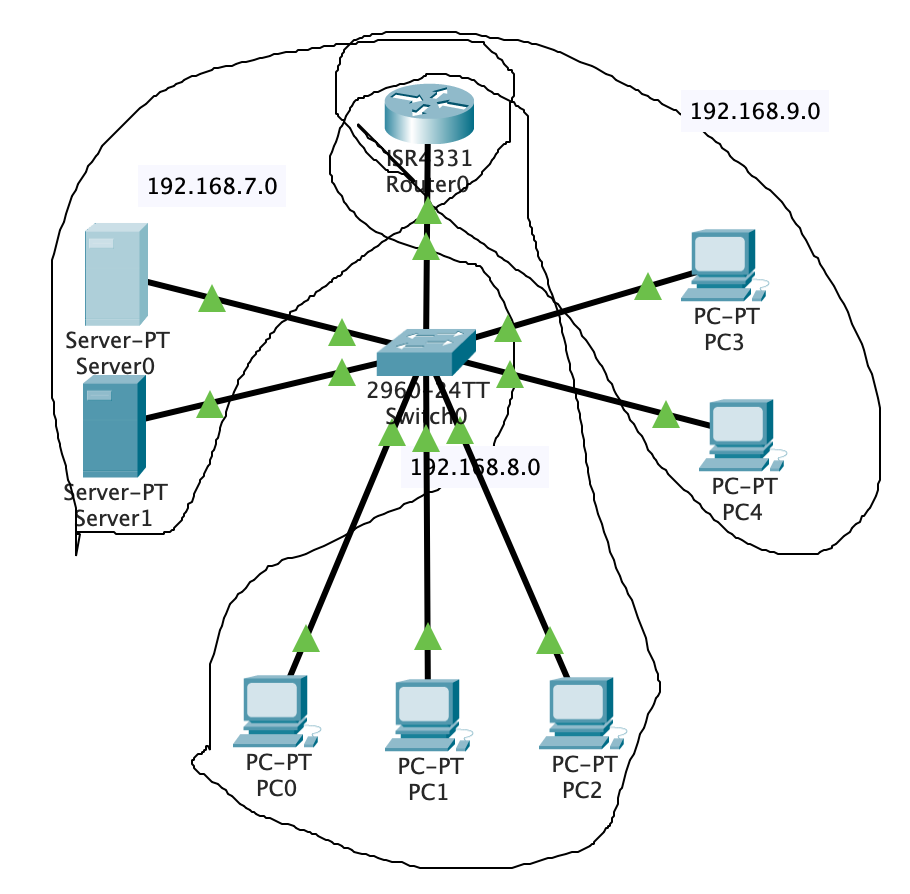
\includegraphics[scale = 0.6]{img/1.png}}
			\caption{Деление на подсети}
			\label{ris:1}
		\end{center}
	\end{figure}

	\section{Настроить поддержку трех виртуальных локальных сетей (VLan 10, 20, 30) на коммутаторе.}
	
	Ниже приведены команды для настройки виртуальных сетей.
	
	int vlan 10
	
	exit
	
	int vlan 20
	
	exit
	
	interface range fa 0/1 - 2
	
	switchport mode access
	
	switchport access vlan 10
	
	exit
	
	interface range fa 0/5 - 7
	
	switchport mode access
	
	switchport access vlan 20
	
	exit
	
	interface range fa 0/3 - 4
	
	switchport mode access
	
	switchport access vlan 30
	
	exit
	
	interface g 0/1
	
	switchport mode trunk
	
	switchport trunk allowed vlan 10
	
	switchport trunk allowed vlan 20
	
	switchport trunk allowed vlan 30

	\begin{figure}[h!]
		\begin{center}
			{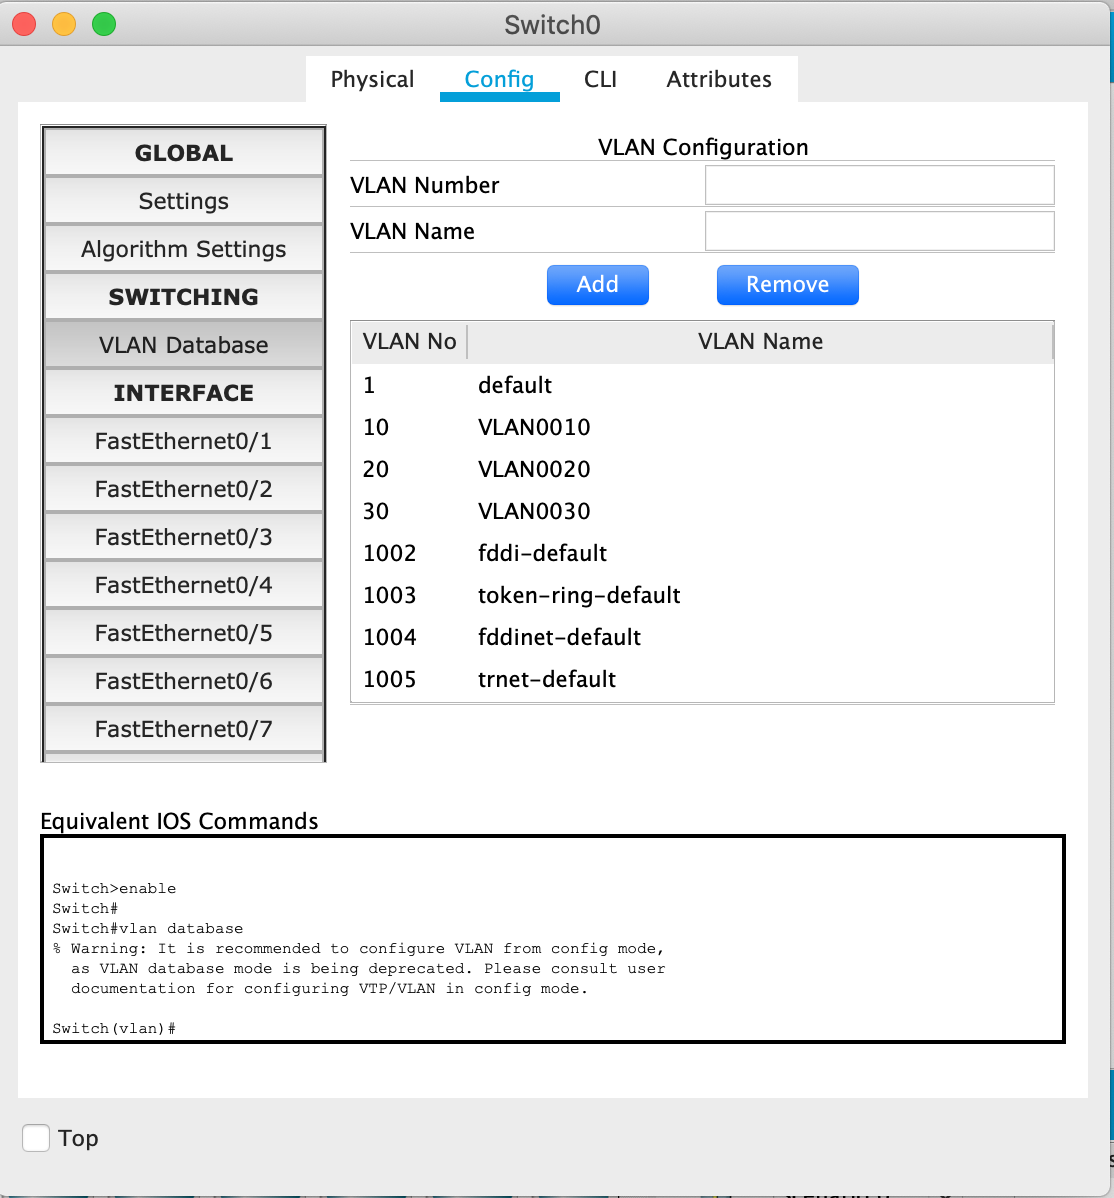
\includegraphics[scale = 0.6]{img/2.png}}
			\caption{ Список виртуальных сетей на коммутаторе}
			\label{ris:2}
		\end{center}
	\end{figure}

	\begin{figure}[h!]
		\begin{center}
			{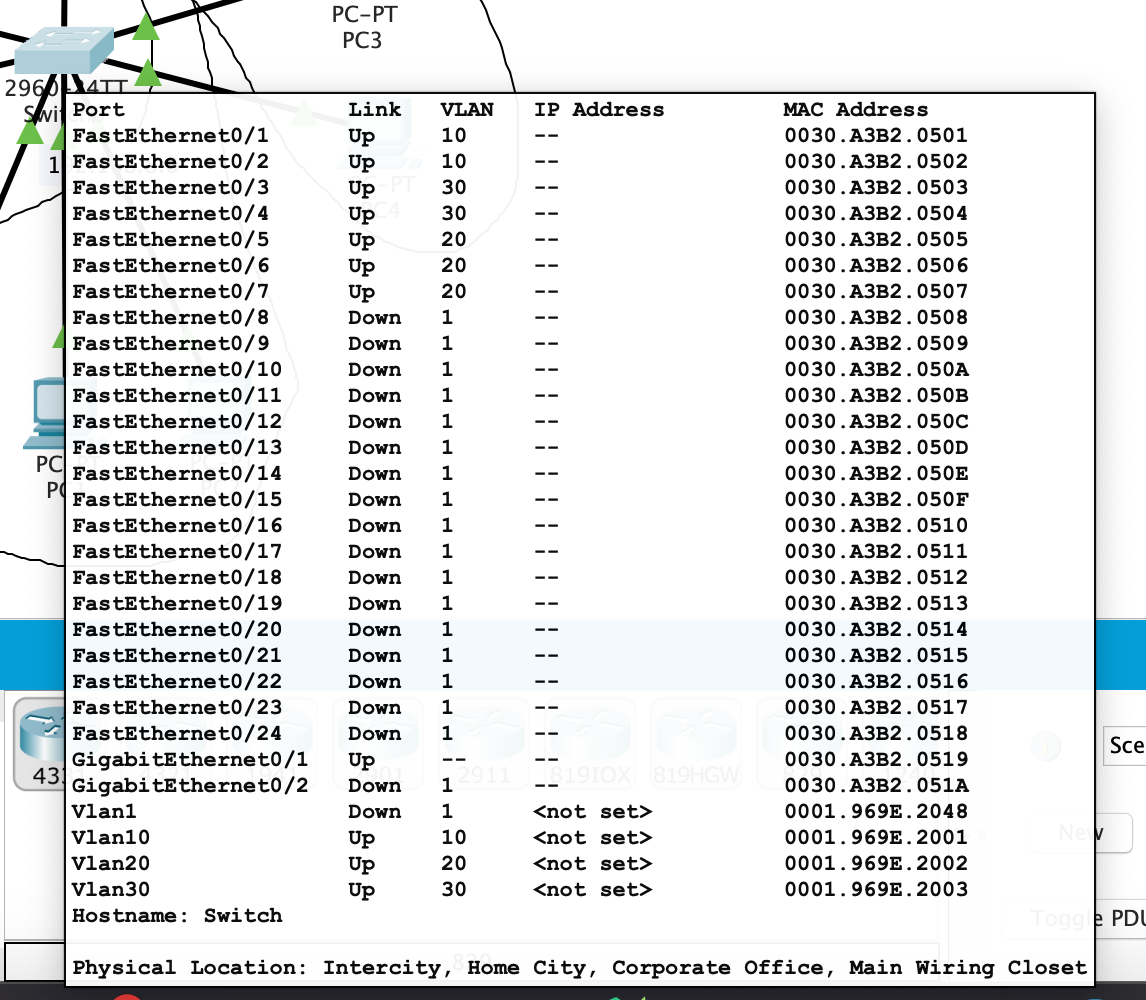
\includegraphics[scale = 0.6]{img/3.png}}
			\caption{Список физических интерфейсов коммутатора}
			\label{ris:3}
		\end{center}
	\end{figure}	

	\section{Настроить маршрутизацию между виртуальными локальными сетями на маршрутизаторе.}

	Ниже приведены команды, которые выполнялись для настройки моршрутизатора.

	int g 0/0/0.1
	
	encapsulation dot1q 10
	
	ip address 192.168.7.254 255.255.255.0
	
	exit
	
	int g 0/0/0.2
	
	encapsulation dot1q 
	
	ip address 192.168.8.254 255.255.255.0
	
	exit
	
	int g 0/0/0.3
	
	encapsulation dot1q 30
	
	ip address 192.168.9.254 255.255.255.0
	
	exit
	
	ip routing
	
	
	\section{Выделить и озаглавить на схеме каждую виртуальную локальную сеть.}
	
	Ниже приведены выделенные виртуальные сети.
	
	\newpage
	
	\begin{figure}[h!]
		\begin{center}
			{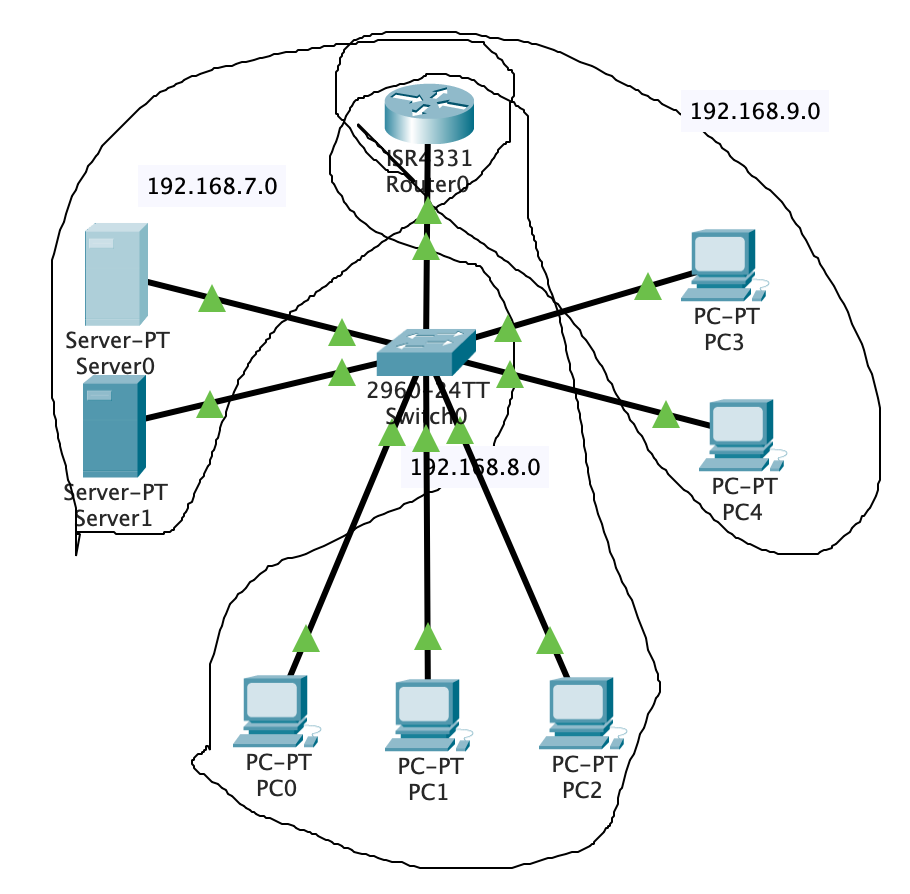
\includegraphics[scale = 0.45]{img/1.png}}
			\caption{Выделенные виртуальные сети}
			\label{ris:5}
		\end{center}
	\end{figure}

	Ниже приведен результат проверки соединения между Server0 и PC3.

	\begin{figure}[h!]
		\begin{center}
			{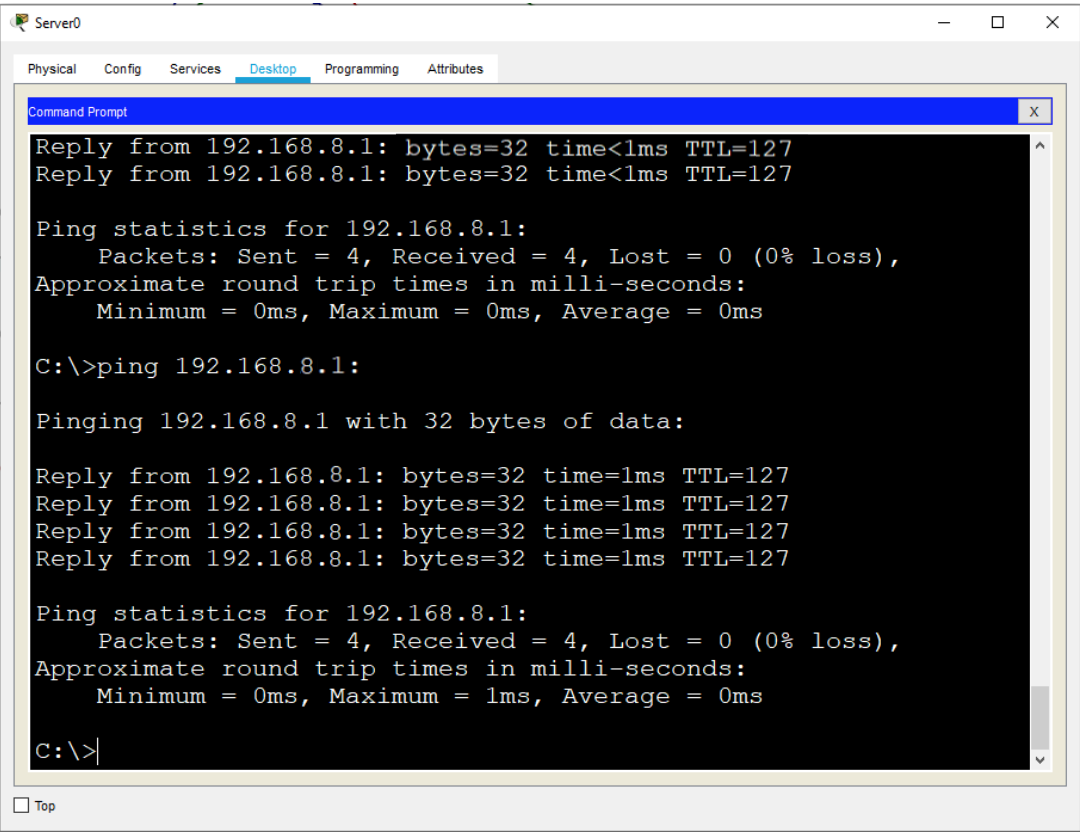
\includegraphics[scale = 0.45]{img/4.png}}
			\caption{Server0 и PC3}
			\label{ris:6}
		\end{center}
	\end{figure}

\end{document}